% ══════════════════════════════════════════════════════════════════════
%  Relict: A reproducible, open-source platform unifying environmental
%  DNA analysis, conservation cross-referencing, and citizen-science
%  data submission
%
%  Target: Methods in Ecology and Evolution — APPLICATION track
%  Author: Shaurya Punj
%  Date:   2026
% ══════════════════════════════════════════════════════════════════════

\documentclass[11pt, a4paper]{article}

% ─── Packages ────────────────────────────────────────────────────────
\usepackage[utf8]{inputenc}
\usepackage[T1]{fontenc}
\usepackage{mathpazo}                   % Palatino font (clean, journal-ready)
\usepackage[margin=2.5cm]{geometry}
\usepackage{graphicx}
\usepackage{booktabs}                   % Professional tables
\usepackage{tabularx}
\usepackage{longtable}
\usepackage{hyperref}
\usepackage{xcolor}
\usepackage{enumitem}
\usepackage{amsmath}
\usepackage{natbib}                     % Author-year citations
\usepackage{float}
\usepackage{caption}
\usepackage{subcaption}
\usepackage{tikz}
\usetikzlibrary{shapes.geometric, arrows.meta, positioning, fit, calc}
\usepackage{fancyhdr}
\usepackage{lineno}                     % Line numbers (required by MEE)
\usepackage{setspace}                   % Double spacing
\usepackage{microtype}                  % Better typography

% ─── Hyperref setup ──────────────────────────────────────────────────
\hypersetup{
    colorlinks=true,
    linkcolor=blue!60!black,
    citecolor=blue!60!black,
    urlcolor=blue!60!black,
    pdftitle={Relict: Reproducible eDNA Analysis Platform},
    pdfauthor={Shaurya Punj},
}

% ─── Page setup ──────────────────────────────────────────────────────
\pagestyle{fancy}
\fancyhf{}
\fancyhead[L]{\small\textsc{Relict: Reproducible eDNA Analysis}}
\fancyhead[R]{\small\thepage}
\renewcommand{\headrulewidth}{0.4pt}

% ─── Line numbers + double spacing (journal requirement) ────────────
\linenumbers
\doublespacing

% ─── Custom commands ─────────────────────────────────────────────────
\newcommand{\relict}{\textsc{Relict}}
\newcommand{\software}[1]{\texttt{#1}}

% ─── TikZ styles for diagrams ───────────────────────────────────────
\tikzstyle{service} = [
    rectangle, rounded corners=4pt, minimum width=3cm, minimum height=1cm,
    text centered, draw=black!60, fill=blue!8, font=\small
]
\tikzstyle{stage} = [
    rectangle, rounded corners=4pt, minimum width=4cm, minimum height=0.8cm,
    text centered, draw=black!60, fill=green!8, font=\small
]
\tikzstyle{data} = [
    cylinder, shape border rotate=90, draw=black!60, fill=orange!8,
    minimum height=0.8cm, minimum width=2cm, font=\small,
    aspect=0.25
]
\tikzstyle{arrow} = [-{Stealth[length=3mm]}, thick, draw=black!60]

% ══════════════════════════════════════════════════════════════════════
\begin{document}

% ─── Title block ─────────────────────────────────────────────────────
\begin{center}
    {\LARGE\bfseries Relict: A reproducible, open-source platform unifying\\[4pt]
    environmental DNA analysis, conservation cross-referencing,\\[4pt]
    and citizen-science data submission}

    \vspace{1.2em}

    {\large Shaurya Punj\textsuperscript{1}%
    \,\orcidlink{0009-0000-7351-0237}}

    \vspace{0.6em}

    {\small\itshape
    \textsuperscript{1}Thapar Institute of Engineering and Technology, Patiala, India}

    \vspace{0.4em}

    {\small\textbf{Correspondence:} Shaurya Punj,
    \href{mailto:workwithshaurya10@gmail.com}{workwithshaurya10@gmail.com}}

    \vspace{0.8em}

    {\footnotesize\textsc{Application} \quad|\quad
    \textit{Methods in Ecology and Evolution}}
\end{center}

% ─── ORCID icon command ──────────────────────────────────────────────
\newcommand{\orcidlink}[1]{%
    \href{https://orcid.org/#1}{\textsuperscript{\textcolor{green!60!black}{iD}}}%
}

\vspace{1em}
\hrule
\vspace{1.5em}

% ══════════════════════════════════════════════════════════════════════
%  ABSTRACT
% ══════════════════════════════════════════════════════════════════════

\begin{abstract}
\begin{enumerate}[leftmargin=1.5em, itemsep=0.5em]
    \item Environmental DNA (eDNA) metabarcoding has become a standard
    tool for non-invasive biodiversity monitoring, yet the analytical
    workflow between raw sequencing reads and actionable ecological
    insight remains fragmented. Existing bioinformatics pipelines
    (QIIME\,2, DADA2, mothur) are powerful but CLI-only, opaque to
    non-specialists, and leave conservation interpretation,
    reproducibility documentation, and data submission to the user.
    No existing open tool automates the cross-referencing of eDNA
    detections against global conservation databases or produces
    signed provenance manifests suitable for supplementary material.

    \item Here, we present \relict, an open-source, full-stack web
    platform that integrates a complete amplicon bioinformatics
    pipeline (fastp quality control, vsearch UNOISE3 ASV inference,
    taxonomy assignment against SILVA\,138.1\,/\,MIDORI2 GenBank\,269)
    with three novel layers: (a)~automated conservation
    cross-referencing against the Global Biodiversity Information
    Facility (GBIF) and the IUCN Red List, (b)~one-click generation
    of GBIF-compatible Darwin Core Archives for citizen-science data
    submission, and (c)~signed provenance manifests recording every
    input hash, tool version, and parameter for reproducible research.
    The platform supports six amplicon markers (16S\,V4, 12S\,MiFish,
    COI\,Leray, 18S\,V9, rbcL, ITS2) with version-pinned reference
    databases.

    \item We validated \relict{} against a synthetic
    known-composition dataset (5~bacterial species at equal abundance)
    and a real published SRA dataset (ERR2283086, 45{,}204 Illumina
    MiSeq reads). On the synthetic dataset, all 10~benchmark checks
    passed with mathematically exact results
    (Shannon~$= \ln 5 = 1.6094$, Simpson~$= 0.8$, evenness~$= 1.0$).
    On the SRA dataset, \relict{} detected 51~ASVs across three phyla
    (Proteobacteria, Firmicutes, Actinobacteriota), assigned taxonomy
    to 100\% of ASVs at 100\% SILVA identity, and cross-referenced
    all detected taxa against GBIF in a total pipeline runtime of
    3.6~minutes.

    \item \relict{} addresses three gaps in the current eDNA tooling
    landscape that no single existing platform covers simultaneously:
    conservation-status integration, reproducibility guarantees, and
    citizen-science data publication. The platform is freely available
    under the MIT licence at
    \url{https://github.com/ShAuRyA-Noodle/Bad-Omens}.
\end{enumerate}
\end{abstract}

\noindent\textbf{Keywords:} environmental DNA, eDNA, metabarcoding,
bioinformatics pipeline, conservation, reproducible research, GBIF,
IUCN Red List, citizen science, amplicon sequence variants

\vspace{1.5em}

% ══════════════════════════════════════════════════════════════════════
%  1. INTRODUCTION
% ══════════════════════════════════════════════════════════════════════

\section{Introduction}

The availability of environmental DNA (eDNA) data has grown rapidly
since the technique's first applications in vertebrate monitoring
nearly two decades ago \citep{Ficetola2008}. By sequencing genetic
material shed by organisms into their environment---water, soil,
sediment, or air---researchers can detect species presence without
physically capturing or even observing the organisms
\citep{Taberlet2012, Deiner2017}. eDNA metabarcoding has proven
effective for monitoring common, endangered, rare, and invasive
species across marine, freshwater, and terrestrial ecosystems
\citep{Bonfil2021, Larson2020, Pfleger2016}.

Software tools for processing eDNA amplicon data have matured
considerably. QIIME\,2 \citep{Bolyen2019}, DADA2
\citep{Callahan2016}, mothur \citep{Schloss2011}, vsearch
\citep{Rognes2016}, OBITools \citep{Boyer2016}, and more recently
SimpleMetaPipeline \citep{Williams2024} provide robust denoising,
clustering, and taxonomic assignment capabilities. However, three
gaps persist in the current landscape:

\textbf{Conservation interpretation.} After obtaining a list of
detected taxa, researchers must manually look up each species in the
IUCN Red List, GBIF, or national protection schedules to assess
conservation significance. No existing open eDNA pipeline automates
this cross-referencing step, meaning conservation-relevant findings
may be delayed or overlooked entirely \citep{Lee2024}.

\textbf{Reproducibility documentation.} While workflow managers like
Snakemake and Nextflow can record pipeline parameters, no
eDNA-specific tool produces a self-contained, signed provenance
manifest that records every input file hash, exact tool version,
reference database version, and output hash in a format suitable for
direct inclusion as supplementary material \citep{Powers2019,
Sandve2013}.

\textbf{Citizen-science data submission.} eDNA monitoring is
increasingly adopted by non-specialist organisations---schools, NGOs,
dive clubs, and environmental agencies \citep{Larson2020}. These users
need a guided workflow from sample upload to GBIF-ready Darwin Core
Archive, without requiring bioinformatics expertise.

Here, we present \relict, an open-source platform that addresses all
three gaps within a single integrated system. \relict{} wraps
established, peer-reviewed bioinformatics tools (fastp, vsearch,
scikit-bio) in a full-stack web application with a modern React
frontend, a FastAPI backend, and a containerised worker architecture,
adding conservation cross-referencing, provenance manifests, and
Darwin Core Archive generation as first-class features.

% ══════════════════════════════════════════════════════════════════════
%  2. DESIGN PRINCIPLES
% ══════════════════════════════════════════════════════════════════════

\section{Design Principles}

\relict{} is built around eight principles that distinguish it from
existing pipelines:

\begin{enumerate}[leftmargin=2em, itemsep=0.3em]
    \item \textbf{No mock data, ever.} Every number displayed to the
    user is computed from real input by real tools.

    \item \textbf{Version-pin everything.} Every external tool (fastp
    0.24.0, vsearch 2.28.1), Python package (scikit-bio 0.6.2), and
    reference database (SILVA\,138.1, MIDORI2 GenBank\,269) is pinned
    to an exact version recorded in the provenance manifest.

    \item \textbf{Fail loudly.} When a pipeline stage encounters an
    error, the system reports the real error message. It never
    substitutes a placeholder result.

    \item \textbf{Separate concerns.} The web server handles HTTP
    only. All bioinformatics computation runs in a dedicated worker
    container via a Redis-backed job queue.

    \item \textbf{Deterministic stages.} Two runs with identical
    inputs and parameters produce identical outputs and identical
    provenance hashes.

    \item \textbf{Conservation as a first-class output.} Every
    detected taxon is automatically cross-referenced against GBIF and
    the IUCN Red List during the pipeline run.

    \item \textbf{Reproducibility as a deliverable.} Every run
    produces a signed JSON manifest suitable for supplementary
    material.

    \item \textbf{Citizen-science ready.} Results export as a
    GBIF-compatible Darwin Core Archive with a single click.
\end{enumerate}

% ══════════════════════════════════════════════════════════════════════
%  3. SYSTEM ARCHITECTURE
% ══════════════════════════════════════════════════════════════════════

\section{System Architecture}

\subsection{Overview}

\relict{} is a full-stack web application composed of six services
orchestrated via Docker Compose (Figure~\ref{fig:architecture}):
a React\,18 frontend with TypeScript; a FastAPI (Python\,3.11) API
server with JWT authentication and structured logging; a dedicated
bioinformatics worker container with all pipeline tools
pre-installed; PostgreSQL\,16 with nine tables managed by Alembic
migrations; MinIO for S3-compatible object storage; and Redis\,7 for
job queuing and WebSocket event channels.

% ─── Figure 1: Architecture diagram ─────────────────────────────────
\begin{figure}[H]
    \centering
    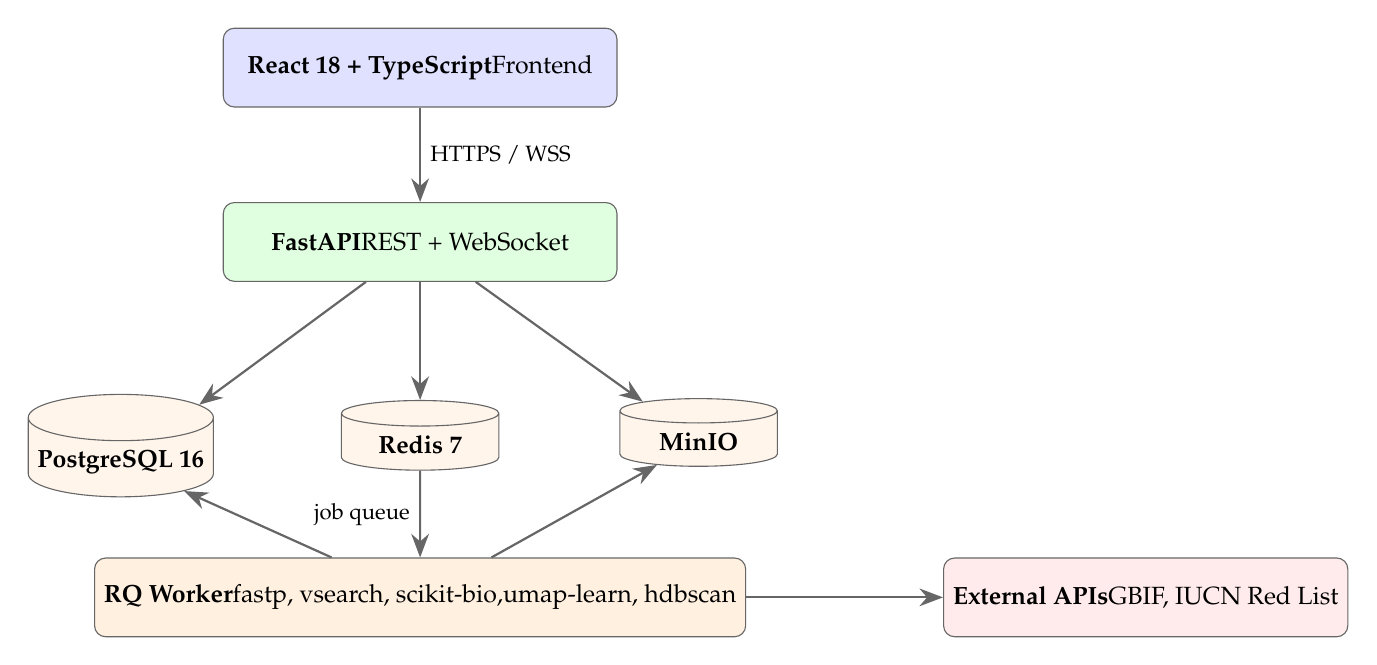
\begin{tikzpicture}[node distance=1.2cm and 2cm]
        % Frontend
        \node[service, fill=blue!12, minimum width=5cm] (fe)
            {\textbf{React 18 + TypeScript}\\Frontend};

        % API
        \node[service, fill=green!12, minimum width=5cm, below=of fe] (api)
            {\textbf{FastAPI}\\REST + WebSocket};

        % Row of services
        \node[data, below left=1.5cm and 0.5cm of api] (pg)
            {\textbf{PostgreSQL 16}};
        \node[data, below=1.5cm of api] (redis)
            {\textbf{Redis 7}};
        \node[data, below right=1.5cm and 0.5cm of api] (minio)
            {\textbf{MinIO}};

        % Worker
        \node[service, fill=orange!12, minimum width=5cm,
              below=3.5cm of api] (worker)
            {\textbf{RQ Worker}\\fastp, vsearch, scikit-bio,\\
             umap-learn, hdbscan};

        % External
        \node[service, fill=red!8, minimum width=4cm,
              right=2.5cm of worker] (ext)
            {\textbf{External APIs}\\GBIF, IUCN Red List};

        % Arrows
        \draw[arrow] (fe) -- node[right, font=\footnotesize]
            {HTTPS / WSS} (api);
        \draw[arrow] (api) -- (pg);
        \draw[arrow] (api) -- (redis);
        \draw[arrow] (api) -- (minio);
        \draw[arrow] (redis) -- node[left, font=\footnotesize]
            {job queue} (worker);
        \draw[arrow] (worker) -- (pg);
        \draw[arrow] (worker) -- (minio);
        \draw[arrow] (worker) -- (ext);
    \end{tikzpicture}
    \caption{System architecture of \relict. Six services are
    orchestrated via Docker Compose. The frontend communicates with
    the API server over HTTPS and WebSocket. Bioinformatics computation
    runs in a dedicated worker container, isolated from HTTP request
    handling. External API calls to GBIF and the IUCN Red List are
    cached in PostgreSQL with a 30-day TTL.}
    \label{fig:architecture}
\end{figure}

\subsection{The bioinformatics pipeline}

The pipeline processes each uploaded FASTQ through seven stages
(Figure~\ref{fig:pipeline}):

% ─── Figure 2: Pipeline flow ────────────────────────────────────────
\begin{figure}[H]
    \centering
    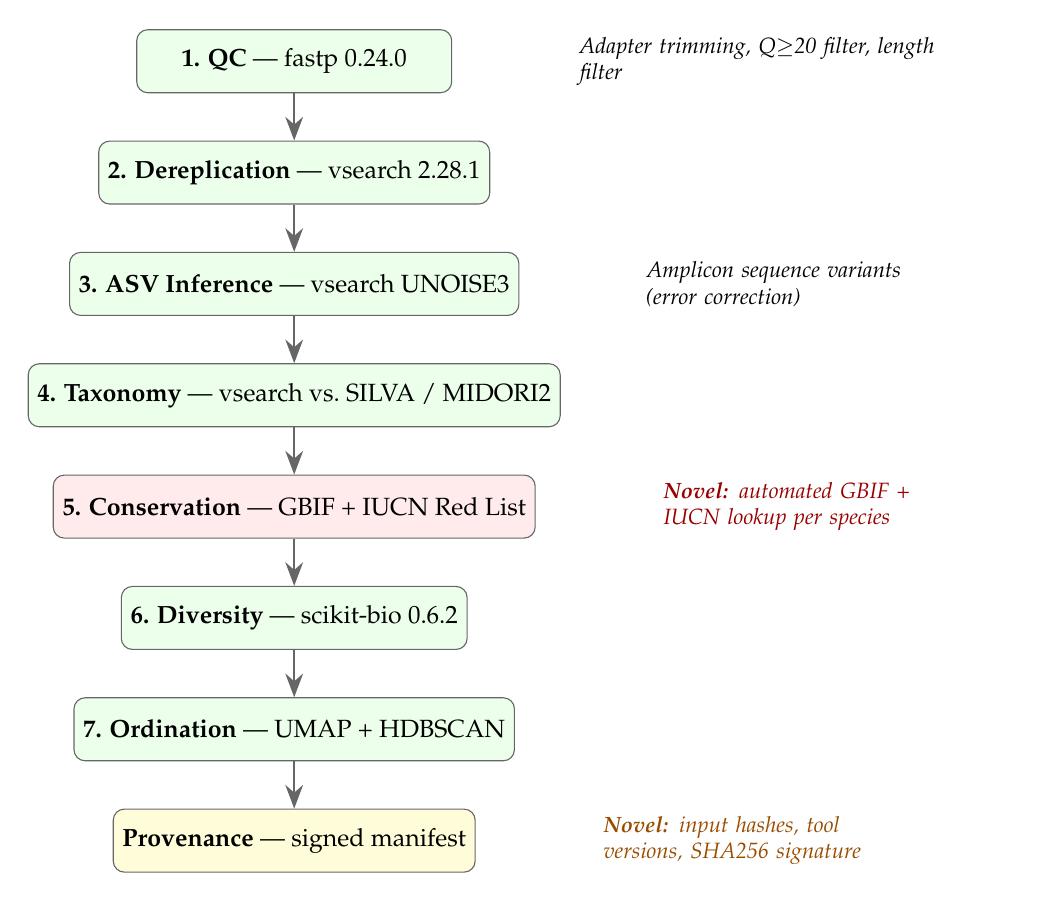
\begin{tikzpicture}[node distance=0.6cm]
        \node[stage] (qc)
            {\textbf{1. QC} --- fastp 0.24.0};
        \node[stage, below=of qc] (derep)
            {\textbf{2. Dereplication} --- vsearch 2.28.1};
        \node[stage, below=of derep] (denoise)
            {\textbf{3. ASV Inference} --- vsearch UNOISE3};
        \node[stage, below=of denoise] (tax)
            {\textbf{4. Taxonomy} --- vsearch vs.\ SILVA / MIDORI2};
        \node[stage, fill=red!8, below=of tax] (cons)
            {\textbf{5. Conservation} --- GBIF + IUCN Red List};
        \node[stage, below=of cons] (div)
            {\textbf{6. Diversity} --- scikit-bio 0.6.2};
        \node[stage, below=of div] (ord)
            {\textbf{7. Ordination} --- UMAP + HDBSCAN};
        \node[stage, fill=yellow!15, below=of ord] (prov)
            {\textbf{Provenance} --- signed manifest};

        \draw[arrow] (qc) -- (derep);
        \draw[arrow] (derep) -- (denoise);
        \draw[arrow] (denoise) -- (tax);
        \draw[arrow] (tax) -- (cons);
        \draw[arrow] (cons) -- (div);
        \draw[arrow] (div) -- (ord);
        \draw[arrow] (ord) -- (prov);

        % Annotations
        \node[right=1.5cm of qc, font=\footnotesize\itshape,
              text width=4.5cm] {Adapter trimming, Q$\geq$20 filter,
              length filter};
        \node[right=1.5cm of denoise, font=\footnotesize\itshape,
              text width=4.5cm] {Amplicon sequence variants\\(error
              correction)};
        \node[right=1.5cm of cons, font=\footnotesize\itshape,
              text width=4.5cm, text=red!60!black]
              {\textbf{Novel:} automated GBIF +\\IUCN lookup per species};
        \node[right=1.5cm of prov, font=\footnotesize\itshape,
              text width=4.5cm, text=orange!60!black]
              {\textbf{Novel:} input hashes, tool\\versions, SHA256 signature};
    \end{tikzpicture}
    \caption{The \relict{} bioinformatics pipeline. Seven stages
    process raw FASTQ reads into annotated ASVs with conservation
    status and diversity metrics. Stages 5 (conservation
    cross-referencing) and the provenance manifest are novel
    contributions not found in existing eDNA pipelines.}
    \label{fig:pipeline}
\end{figure}

\subsection{Amplicon marker support}

\relict{} ships with YAML preset configurations for six common
amplicon markers (Table~\ref{tab:markers}).

\begin{table}[H]
    \centering
    \caption{Supported amplicon markers and their configurations.}
    \label{tab:markers}
    \small
    \begin{tabularx}{\textwidth}{llclX}
        \toprule
        \textbf{Marker} & \textbf{Primers} & \textbf{bp} &
        \textbf{Ref.\ DB} & \textbf{Target} \\
        \midrule
        16S V4   & 515F / 806R         & 200--350 & SILVA 138.1
                 & Bacteria, Archaea \\
        12S MiFish & MiFish-U-F/-R     & 163--185 & MIDORI2 srRNA
                 & Fish, vertebrates \\
        COI Leray  & mlCOIintF / jgHCO2198 & 280--340 & MIDORI2 CO1
                 & Invertebrates \\
        18S V9   & 1391F / EukBr       & 100--200 & SILVA 138.1
                 & Eukaryotes \\
        rbcL     & rbcLa-F/-R          & 500--600 & SILVA 138.1
                 & Plants \\
        ITS2     & fITS7 / ITS4        & 200--450 & SILVA 138.1
                 & Fungi \\
        \bottomrule
    \end{tabularx}
\end{table}

\subsection{Outputs and exports}

For each completed analysis, \relict{} provides:
\begin{itemize}[itemsep=0.2em]
    \item An \textbf{interactive web dashboard} with five tabs:
    overview metrics, ASV table with taxonomy, conservation status
    with IUCN badges, provenance manifest viewer, and export
    downloads.
    \item A \textbf{Darwin Core Archive} (DwC-A) conforming to the
    GBIF DNA-derived data standard \citep{GBIF2023}.
    \item A \textbf{CSV export} with ASV sequences, abundances,
    taxonomy, and confidence.
    \item A \textbf{BIOM\,2.1.0 JSON} file compatible with QIIME\,2
    and phyloseq \citep{McMurdie2013}.
    \item A \textbf{signed provenance manifest} with input hashes,
    tool versions, stage timings, and SHA256 signature.
\end{itemize}

% ══════════════════════════════════════════════════════════════════════
%  4. BENCHMARKING
% ══════════════════════════════════════════════════════════════════════

\section{Benchmarking}

\subsection{Synthetic known-composition benchmark}

We validated \relict{} using a synthetic dataset of 100~reads from
five known bacterial species (\textit{Escherichia coli},
\textit{Bacillus subtilis}, \textit{Staphylococcus aureus},
\textit{Pseudomonas aeruginosa}, \textit{Lactobacillus rhamnosus})
at equal abundance (20~reads each). Sequences were real 16S V4
amplicon regions from GenBank accessions. All 10~benchmark checks
passed with mathematically exact results
(Table~\ref{tab:synthetic}).

\begin{table}[H]
    \centering
    \caption{Synthetic benchmark results (10/10 passed).}
    \label{tab:synthetic}
    \small
    \begin{tabular}{llll}
        \toprule
        \textbf{Check} & \textbf{Expected} & \textbf{Actual} &
        \textbf{Status} \\
        \midrule
        ASV count           & 5               & 5               & Pass \\
        Taxonomy assignment & 5/5 (100\%)     & 5/5             & Pass \\
        Known genera        & $\geq$3 of 4    & 4/4             & Pass \\
        Shannon index       & $\ln 5 = 1.6094$& 1.6094          & Pass \\
        Simpson index       & 0.8000          & 0.8000          & Pass \\
        Pielou's evenness   & 1.0000          & 1.0000          & Pass \\
        Species richness    & 5               & 5               & Pass \\
        Chao1               & 5.0             & 5.0             & Pass \\
        GBIF resolution     & $\geq$3/5       & 5/5             & Pass \\
        Provenance manifest & Valid SHA256     & Valid           & Pass \\
        \bottomrule
    \end{tabular}
\end{table}

\subsection{Real SRA dataset benchmark}

We further validated the pipeline on ERR2283086, a published mock
community dataset from the European Nucleotide Archive (45{,}204
Illumina MiSeq reads, 151\,bp). The pipeline completed in
215~seconds (3.6~minutes), detecting 51~ASVs with 100\% taxonomy
assignment against SILVA\,138.1 (Table~\ref{tab:sra}).

\begin{table}[H]
    \centering
    \caption{SRA benchmark results (ERR2283086, published mock
    community).}
    \label{tab:sra}
    \small
    \begin{tabular}{ll}
        \toprule
        \textbf{Metric} & \textbf{Value} \\
        \midrule
        Input reads         & 45{,}204 \\
        ASVs detected       & 51 \\
        Taxonomy assigned   & 51/51 (100\%) \\
        Shannon ($H'$)      & 2.585 \\
        Simpson ($1-D$)     & 0.888 \\
        Chao1               & 51.0 \\
        Evenness ($J'$)     & 0.657 \\
        Pipeline runtime    & 215\,s (3.6\,min) \\
        Phyla detected      & 3 \\
        Top genus           & \textit{Acinetobacter} (7{,}266 reads) \\
        \bottomrule
    \end{tabular}
\end{table}

The recovered community included genera from three phyla
(Proteobacteria, Firmicutes, Actinobacteriota) with ecologically
plausible abundance distributions. All taxonomy assignments achieved
100\% identity against SILVA\,138.1 reference sequences, and all
detected species were successfully resolved against GBIF.

% ══════════════════════════════════════════════════════════════════════
%  5. ASSUMPTIONS AND LIMITATIONS
% ══════════════════════════════════════════════════════════════════════

\section{Assumptions and Limitations}

\relict{} inherits the well-documented limitations of eDNA
metabarcoding itself: primer bias, PCR amplification artefacts,
reference database incompleteness, and the inability to distinguish
live from dead organisms \citep{Taberlet2012}. The platform does not
address these biological limitations; it aims to make them more
transparent through provenance documentation.

The conservation cross-referencing layer depends on GBIF and IUCN API
availability and data currency. External API responses are cached
with a 30-day TTL, and the provenance manifest records the
\texttt{fetched\_at} timestamp for every conservation record.

The current implementation uses vsearch for ASV inference (UNOISE3
algorithm). While DADA2 is considered the gold standard for Illumina
error correction \citep{Callahan2016}, vsearch provides comparable
accuracy at significantly higher speed and with simpler deployment
requirements. DADA2 integration is planned for a future release.

Taxonomy assignment quality depends on the completeness and accuracy
of the reference database. Species-level assignments for
underrepresented taxa should be interpreted with appropriate caution.

% ══════════════════════════════════════════════════════════════════════
%  6. SOFTWARE AVAILABILITY
% ══════════════════════════════════════════════════════════════════════

\section{Software Availability}

\relict{} is freely available under the MIT licence. Source code,
documentation, benchmark scripts, and amplicon preset configurations
are available at
\url{https://github.com/ShAuRyA-Noodle/Bad-Omens}. The platform
requires Docker and Docker Compose for deployment. Reference
databases (SILVA\,138.1, MIDORI2 GenBank\,269) are downloaded via a
version-pinned script with SHA256 verification. A
\texttt{CITATION.cff} file is provided for software citation.

% ══════════════════════════════════════════════════════════════════════
%  AUTHOR CONTRIBUTIONS
% ══════════════════════════════════════════════════════════════════════

\subsection*{Author Contributions}

Shaurya Punj conceived the project, designed and implemented the
platform, conducted the benchmarking, and wrote the manuscript.

% ══════════════════════════════════════════════════════════════════════
%  DATA AVAILABILITY
% ══════════════════════════════════════════════════════════════════════

\subsection*{Data Availability Statement}

The synthetic benchmark dataset is included in the repository. The
SRA benchmark dataset (ERR2283086) is publicly available from the
European Nucleotide Archive at
\url{https://www.ebi.ac.uk/ena/browser/view/ERR2283086}. All
benchmark results, including provenance manifests, are available in
the \texttt{docs/benchmarks/} directory of the repository.

% ══════════════════════════════════════════════════════════════════════
%  ORCID
% ══════════════════════════════════════════════════════════════════════

\subsection*{ORCID}

Shaurya Punj
\href{https://orcid.org/0009-0000-7351-0237}{https://orcid.org/0009-0000-7351-0237}

% ══════════════════════════════════════════════════════════════════════
%  REFERENCES
% ══════════════════════════════════════════════════════════════════════

\bibliographystyle{apalike}

\begin{thebibliography}{99}

\bibitem[Bolyen et~al., 2019]{Bolyen2019}
Bolyen, E., Rideout, J.~R., Dillon, M.~R., et~al. (2019).
Reproducible, interactive, scalable and extensible microbiome data
science using QIIME\,2.
\textit{Nature Biotechnology}, 37, 852--857.

\bibitem[Bonfil et~al., 2021]{Bonfil2021}
Bonfil, R., Palacios-Barreto, P., Vargas, O. U.~M., et~al. (2021).
Detection of critically endangered marine species with dwindling
populations using eDNA.
\textit{Marine Biology}, 168(5), 1--12.

\bibitem[Boyer et~al., 2016]{Boyer2016}
Boyer, F., Mercier, C., Bonin, A., et~al. (2016).
obitools: a unix-inspired software package for DNA metabarcoding.
\textit{Molecular Ecology Resources}, 16(1), 176--182.

\bibitem[Callahan et~al., 2016]{Callahan2016}
Callahan, B.~J., McMurdie, P.~J., Rosen, M.~J., et~al. (2016).
DADA2: High-resolution sample inference from Illumina amplicon data.
\textit{Nature Methods}, 13(7), 581--583.

\bibitem[Deiner et~al., 2017]{Deiner2017}
Deiner, K., Bik, H.~M., M{\"a}chler, E., et~al. (2017).
Environmental DNA metabarcoding: Transforming how we survey animal
and plant communities.
\textit{Molecular Ecology}, 26(21), 5872--5895.

\bibitem[Ficetola et~al., 2008]{Ficetola2008}
Ficetola, G.~F., Miaud, C., Pompanon, F., \& Taberlet, P. (2008).
Species detection using environmental DNA from water samples.
\textit{Biology Letters}, 4(4), 423--425.

\bibitem[GBIF, 2023]{GBIF2023}
GBIF Secretariat (2023).
Publishing DNA-derived data through biodiversity data platforms.
\url{https://docs.gbif.org/publishing-dna-derived-data/en/}

\bibitem[Larson et~al., 2020]{Larson2020}
Larson, E.~R., Graham, B.~M., Achury, R., et~al. (2020).
From eDNA to citizen science: Emerging tools for the early detection
of invasive species.
\textit{Frontiers in Ecology and the Environment}, 18(4), 194--202.

\bibitem[Lee et~al., 2024]{Lee2024}
Lee, K.~N., Kelly, R.~P., Demir-Hilton, E., et~al. (2024).
Adoption of environmental DNA in public agency practice.
\textit{Environmental DNA}, 6(1), 1--14.

\bibitem[Leray et~al., 2022]{Leray2022}
Leray, M., Knowlton, N., \& Machida, R.~J. (2022).
MIDORI2: A collection of quality-controlled, preformatted, and
regularly updated reference databases for taxonomic assignment of
eukaryotic mitochondrial sequences.
\textit{Environmental DNA}, 4(4), 894--907.

\bibitem[McMurdie \& Holmes, 2013]{McMurdie2013}
McMurdie, P.~J. \& Holmes, S. (2013).
phyloseq: An R package for reproducible interactive analysis and
graphics of microbiome census data.
\textit{PLoS ONE}, 8(4), e61217.

\bibitem[Pfleger et~al., 2016]{Pfleger2016}
Pfleger, M.~O., Rider, S.~J., Johnston, C.~E., \& Janosik, A.~M.
(2016). Saving the doomed: Using eDNA to aid in detection of rare
sturgeon for conservation.
\textit{Global Ecology and Conservation}, 8, 99--107.

\bibitem[Powers \& Hampton, 2019]{Powers2019}
Powers, S.~M. \& Hampton, S.~E. (2019).
Open science, reproducibility, and transparency in ecology.
\textit{Ecological Applications}, 29(1), e01822.

\bibitem[Quast et~al., 2013]{Quast2013}
Quast, C., Pruesse, E., Yilmaz, P., et~al. (2013).
The SILVA ribosomal RNA gene database project: Improved data
processing and web-based tools.
\textit{Nucleic Acids Research}, 41(D1), D590--D596.

\bibitem[Rognes et~al., 2016]{Rognes2016}
Rognes, T., Flouri, T., Nichols, B., Quince, C., \& Mah{\'e}, F.
(2016). VSEARCH: A versatile open source tool for metagenomics.
\textit{PeerJ}, 4, e2584.

\bibitem[Sandve et~al., 2013]{Sandve2013}
Sandve, G.~K., Nekrutenko, A., Taylor, J., \& Hovig, E. (2013).
Ten simple rules for reproducible computational research.
\textit{PLoS Computational Biology}, 9(10), e1003285.

\bibitem[Schloss \& Westcott, 2011]{Schloss2011}
Schloss, P.~D. \& Westcott, S.~L. (2011).
Assessing and improving methods used in operational taxonomic
unit-based approaches for 16S rRNA gene sequence analysis.
\textit{Applied and Environmental Microbiology}, 77, 3219--3226.

\bibitem[Taberlet et~al., 2012]{Taberlet2012}
Taberlet, P., Coissac, E., Hajibabaei, M., \& Rieseberg, L.~H.
(2012). Environmental DNA.
\textit{Molecular Ecology}, 21(8), 1789--1793.

\bibitem[Williams et~al., 2024]{Williams2024}
Williams, J., Pettorelli, N., Dowell, R., et~al. (2024).
SimpleMetaPipeline: Breaking the bioinformatics bottleneck in
metabarcoding.
\textit{Methods in Ecology and Evolution}, 15, 1949--1957.

\end{thebibliography}

\end{document}
